% Chapter 2

\chapter{Funzioni elementari} % Chapter title

\label{ch:funzioni-elementari} % For referencing the chapter elsewhere, use \autoref{ch:introduction} 

%----------------------------------------------------------------------------------------

\subsection{Polinomi}
\[f(x)=a_0+a_1 x + \dots + a_n x^n =\displaystyle\sum_{k=0}^{n} a_k x^k \]
\[a_0, a_1, \dots, a_n \in \R \text{ Coefficienti}\qquad a_n \neq 0 \text{ n è il grado del polinomio}\]

Per cui:
\[n=1 \qquad y=a_0+a_1 x \quad \text{Rette}\]
\[n=2 \qquad y=a_0+a_1 x + a_2 x^2 \quad \text{Parabole}\]
\subsection{Potenze}
Fissato un esponente $a \in \R$ la funzione potenza è:
\[f(x)=x^a\]
la cui definizione e dominio dipendono dal valore dell’esponente a.
\begin{itemize}
\item $a=n \in \N$
\[f(x)=x^n= \underbrace{x \times \dots \times x}_{\textbf{n volte}} \qquad \dom f=\R \qquad \im f= 
\begin{cases}
		\R \qquad \text{se n dispari} \\
		[0,+\infty )  \qquad \text{se n pari } n \neq 0 \\
		\{0\}  \qquad n = 1
\end{cases}\]

\item $a=-n\in \Z , n\in \N ,n \geq 1$
\[f(x)=x^{-n}=\frac{1}{x^n} \qquad \dom f = \R \backslash \{0\} \qquad \im f=
\begin{cases}
		\R \backslash \{0\} \qquad \text{n dispari} \\
		(0,+\infty )  \qquad \text{n pari }
\end{cases}
\]
\item $a=\frac{1}{n} \in \Z , n\in \N ,n \geq 2$
\[f(x)=x^{\frac{1}{n}}=\sqrt[n]{x} \qquad 
\dom f = 
\begin{cases}
		\R \qquad \text{n dispari} \\
		[0,+\infty )  \qquad \text{n pari }
\end{cases}
\qquad \im f=
\begin{cases}
		\R \qquad \text{n dispari} \\
		[0,+\infty) \qquad \text{n pari }
\end{cases}
\]

\item $a=\frac{m}{n} \in \Q , n\in \N ,n \geq 1 , m \in \Z$
\[f(x)=x^{\frac{m}{n}}=\sqrt[n]{m} \qquad 
\dom f = (0,+\infty)
\qquad \im f=(0,+\infty)\]

\item $a \in \R$
\[f(x)=x^a=
\begin{cases}
	\text{sup}\{x^q | q \in \Q , q \leq a\} \quad x \geq 1 \\
	\text{inf} \{x^q | q\in \Q , q \leq a\} \quad 0 < x < 1
\end{cases}
\qquad
\dom f = (0, + \infty)
\qquad
\im f = (0, + \infty)
\]


\end{itemize}

\begin{figure}[bth]
\myfloatalign
\subfloat[Potenze.]
{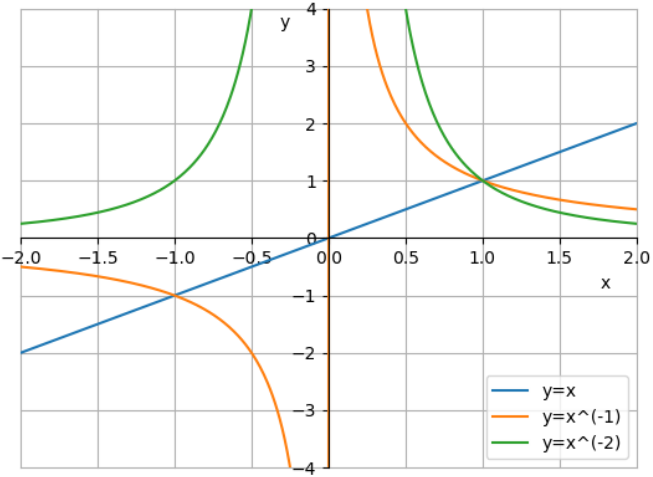
\includegraphics[width=.45\linewidth]{gfx/images/potenze.png}} 
\end{figure}
Osserviamo che:
\begin{itemize}
	\item $f(0)=0$
	\item $f(1)=1$
	\item se $n$ pari $f$ è pari
	\item se $n$ dispari $f$ è dispari
\end{itemize}

\subsubsection{Proprietà delle potenze}
\begin{itemize}
\item $x^{n+m}=x^n x^m$
\item $(x^n)^m=x^{nm}$
\end{itemize}

\paragraph{Osservazioni}
\[f(x)=x^0=1 \quad \forall x \in \R\]
\[0^0=1\]

\paragraph{Dimostrazioni}

\[x^{n+m}= \underbrace{x \times \dots \times x}_{\text{n+m volte}}=\underbrace{(x \times \dots \times x)}_{\text{n volte}}\times \underbrace{x \times \dots \times x}_{\text{m volte}}=x^{n+m}\]

\[(x^{n})^m= \underbrace{x^n \times \dots \times x^n}_{\text{m volte}}\]

\[x^n=x^{n+0}=x^n x^0 \qquad x\neq 0\]
\[x^0 = 1 \quad \forall x \in \R\]

\subsection{Esponenziale}
Fissata la base $a>0$ con $a \neq 1$, la funzione esponenziale è
\[f(x)=a^x \qquad \dom f = \R \qquad \im f = (0,+\infty)\]
Se si sceglie come base il numero di Nepero $e=2.71828\dots > 1$, la funzione esponenziale si denota:
\[f(x)=e^x=\exp x\]

\subsubsection{Proprietà}
\begin{enumerate}
	\item se $a>1$, allora la funzzione $a^x$ è strettamente crescente
	\item se $0<a<1$, allora la funzione $a^x$ è strettamente decrescente
	\item se $0<a<b$ con $a,b \neq 1$
	\[\begin{cases}
		a^x<b^x \qquad x>0 \\
		a^x > b^x \qquad x<0
	\end{cases}\]
	\item valgono le seguenti proprietà:
	\begin{itemize}
	\item $a^0=1$
	\item $a^1=a$
	\item $a^{x_1+x_2}=a^{x_1+x_2} \qquad x_1,x_2 \in \R$
	\item $a^{-x}=(\frac{1}{a})^x \qquad x \in \R$
	\item $(a^x)^b = a^{bx} \qquad x,b \in \R$
	\end{itemize}
\end{enumerate}

\begin{figure}[bth]
\myfloatalign
\subfloat[Esponenziali.]
{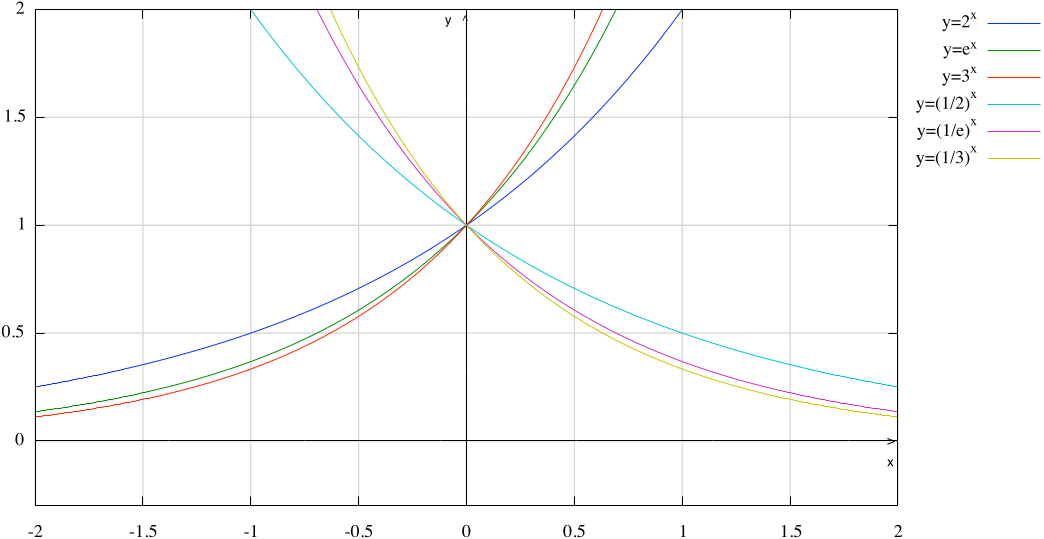
\includegraphics[width=.45\linewidth]{gfx/images/esponenziali.png}} 
\end{figure}

\subsection{Logaritmo}
Fissata la base $a>0$ con $a\neq 1$, la funzione logaritmo
\[f(x)=\log_a x \qquad \dom f = (0,+\infty) \qquad \im f = \R\]
è definita come la funzione inversa della funzione esponenziale $a^x$. Se si sceglie come base il numero di Nepero \textit{e}, il logaritmo si denota:
\[f(x)=\log_e = \log x = \ln x\]

\begin{enumerate}
	\item se $a>1$, allora la funzione $\log_a x$ è strettamente crescente
	\item se $0<a<1$, allora la funzione $\log_a x$ è strettamente decrescente
	\item se $0<a<b$ con $a,b\neq 1$
	\[\begin{cases}
	\log_a x > \log_b x \qquad se x>1 \\
	\log_a x < \log_b x \qquad se 0<x<1 \\
	\end{cases}\]
	\item valgono le seguenti proprietà:
	\begin{itemize}
		\item $\log_a a^x = x \qquad x>1$
		\item $a^{\log_a x}=x \qquad x>0$
		\item $\log_a 1 = 0$
		\item $\log_a a = 1$
		\item $\log_a (x_1 x_2)= \log_a x_1 + \log_a x_2 \qquad x_1,x_2 > 0$
		\item $\log_a (\frac{x_1}{x_2})=\log_a x_1 - \log_a x_2 \qquad x_1,x_2 > 0$
		\item $\log_a x^b = b \log_a x \qquad x>0, b \in \R$
		\item $\log_a x= \frac{\log_b x}{\log_b a}=\frac{\ln x}{\ln a}\qquad x>0,b>0,b\neq 1$
		\item $a^x = e^{(\ln a)x} \qquad x\in \R, a>0, a \neq 1$
	\end{itemize}
\end{enumerate}

\begin{figure}[bth]
\myfloatalign
\subfloat[Logaritmi.]
{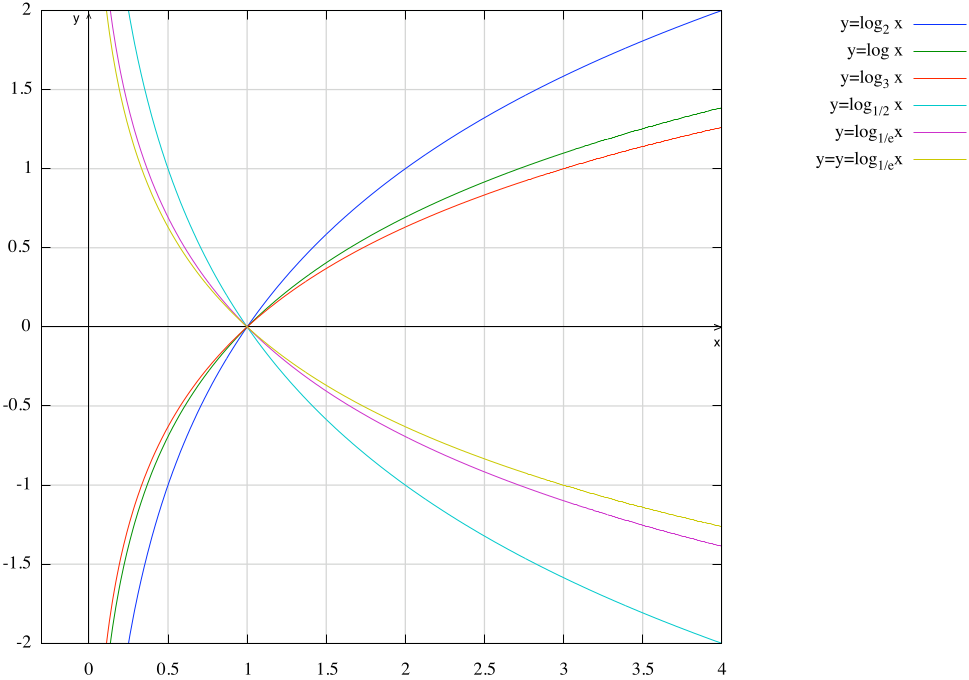
\includegraphics[width=.45\linewidth]{gfx/images/logaritmi.png}} 
\end{figure}

\section{Funzioni trigonometriche}
Una funuone $f:\R \in \R$ è detta periodica di periodo $T$, $T>0$ se:
\[f(x+T)=f(x) \forall x \in \R\]
La caratteristica fondamentale delle funzioni periodiche è che i suoi valori si ripetono dopo intervalli di ampiezza $T$.

\subsection{Le funzioni seno e coseno}
Sia $\gamma$ una circonferenza di raggio $1$ (detta circonferenza goniometrica) il cui centro $O$ è anche l'origine di un sistema di assi cartesiani e sia $A$ il punto $(1,0)$.
Partendo da $A$ percorriamo la circonferenza in senso antiorario oppure in senso orario.
Sia $x$ un numero reale, denotiamo con $P_x$ il punto su $\gamma$ che si ottiene percorrendo la circonferenza a partire dal punto $A$ per un arco di lunghezza $|x|$, in senso antorario se $x \geq 0$, oppure in senso orario se $x<0$.
Il punto $P_x$ individua un angolo nel piano avente vertice $O$ e delimitatio dalle semirette nel piano uscenti da $O$ e passanti per $A$ e per $P_x$.
Il numero reale $x$ rappresenta la misura dell'angolo in radianti.


\begin{figure}[bth]
\myfloatalign
\subfloat[Circonferenza goniometrica con seno e coseno.]
{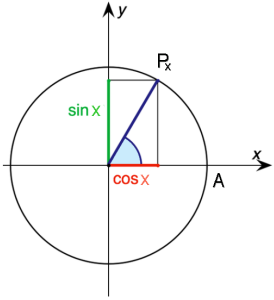
\includegraphics[width=.45\linewidth]{gfx/circonferenza.png}} 
\end{figure}



Osserviamo che l'incremento della lunghezza $x$ di $2\pi$ corrisponde a compiere un intero giro sulla circonferenza in senso antiorario ritornando al punto $P_x$ (così come decrementare di $2\pi$ la lunghezza $x$). Quindi si ha:
\[P_{x\pm k2\pi}=P_x \qquad \forall x \in \R, k \in \N\]

\paragraph{Simmetria}
Indichiamo con $\cos x$ e con $\sin x$ rispettivamente l'ascissa e l'ordinata del punto $P_x$. Le funzioni $y=\cos x$ e $y=\sin x$ sono definite su $\R$ a valori nell'intervallo $[-1,1]$, sono periodiche di minimo periodo $2\pi$ e soddisfano la relazione:
\[\sin^2 x + \cos^2 x = 1\]

\paragraph{Monotonia} Per la periodicità di seno e coseno ci basta studiarne le proprietà nell'intervallo $[0,2\pi]$. Dalle definizioni segue subito che la funzione seno è dispari e la funzione coseno è pari; inoltre la funzione coseno è strettamente decrescente in $[0,\pi]$ e strettamente crescente in $[\pi,2\pi]$. La funzione seno è strettamente crescente in $[0,\frac{\pi}{2}] \cup [\frac{3}{2}\pi,2\pi)$ e strettamente decrescente in $[\frac{\pi}{2},\frac{3}{2}\pi]$.

\begin{figure}[bth]
\myfloatalign
\subfloat[Grafico delle funzioni: seno (sinistra) e coseno (destra).]
{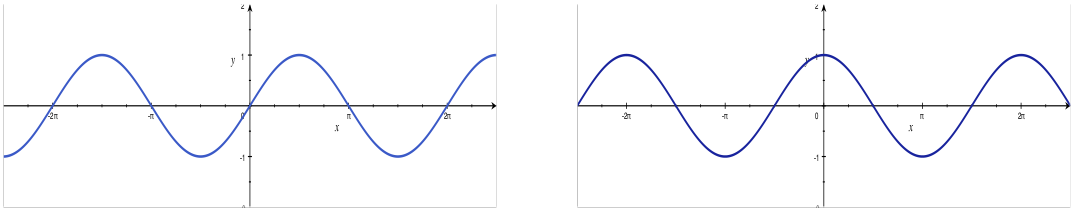
\includegraphics[width=.45\linewidth]{gfx/images/senocoseno.png}} 
\end{figure}

\subsubsection{Formule trigonometriche}
\paragraph{Formule di addizione e sottrazione}
\[\sin(\alpha\pm\beta)=\sin(\alpha)\cos(\beta)\pm\cos(\alpha)\sin(\beta)\]
\[\cos(\alpha\pm\beta)=\cos(\alpha)\cos(\beta)\mp\sin(\alpha)\sin(\beta)\]
\paragraph{Formule di duplicazione}
\[\sin(2x)=2\sin x\cos x\]
\[\cos(2x)=2\cos^2 x - 1\]
\paragraph{Formule di potenza}
\[(\sin x)^2 = \sin^2 x= \frac{1-\cos(2x)}{2}\]
\[(\cos x)^2 = \cos^2 x= \frac{1+\cos(2x)}{2}\]
\paragraph{Formule di bisezione}
\[\sin(\frac{x}{2})=\sqrt{\frac{1-\cos x}{2}} \qquad 0<x\leq 2\pi\]
\[\cos(\frac{x}{2})=\sqrt{\frac{1+\cos x}{2}} \qquad -\pi<x\leq \pi\]
\paragraph{Formule di prostaferesi}
\[\sin x -\sin y=2\sin(\frac{x-y}{2})\cos(\frac{x+y}{2})\]
\[\cos x -\cos y=-2\cos(\frac{x-y}{2})\sin(\frac{x+y}{2})\]


\[\cos(x+\pi)=-\cos x \qquad \sin(x+\pi)=-\sin x\]
\[\cos(x+\frac{\pi}{2})=-\sin x \qquad \sin(x+\frac{\pi}{2})=\cos x \]

\subsection{La funzione tangente e la funzione cotangente}
La funzione tangente è:
\[\tan x = \frac{\sin x}{\cos x}\]
è definita nei punti di $\R$ diversi da $\frac{\pi}{2} +k\pi,k\in\Z$ e, come vedremo in seguito, ha immagine $\R$.

\subsubsection{Proprietà fondamentali}
Dal grafico della tangente di ottiene che $\tan(x)=\tan(x+k\pi)$ per $k\in \Z$ cioè $\tan(x)$ è periodica di minimo periodo $T=\pi$

\begin{figure}[bth]
\myfloatalign
\subfloat[Funzioni trigonometriche.]
{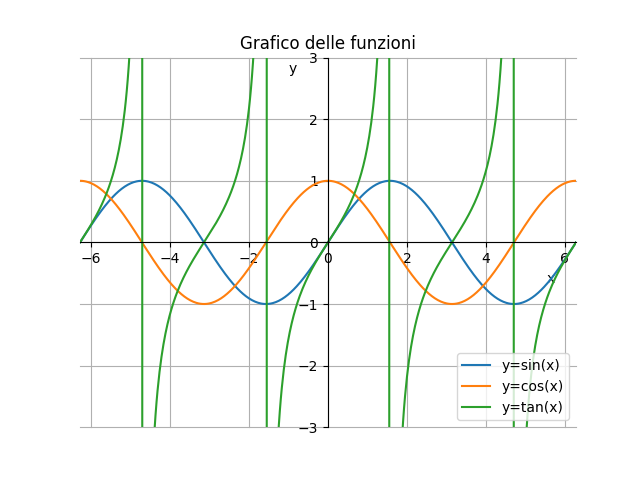
\includegraphics[width=.45\linewidth]{gfx/images/trigonometriche.png}} 
\end{figure}